Conditional Network Embedding (CNE) is a node embedding method for
graphs that has been successfully applied to visualization and
prediction. It allows the user to generate embeddings that respect the
network structure, while factoring out prior knowledge known in advance.
Applications of this include visualizing the nodes in a network without
representing undesired effect, such as for instance having the high
degree nodes concentrated in the center of the embedding space. Such
embeddings can also be used to predict links while controlling the
influence of sensitive node attributes on the predictions. This has
great interest in producing fair link prediction on social networks for
instance.

In what follows we aim to give a comprehensive view of the underlying
mechanism that make CNE good at producing embeddings that factor out
prior information.

\hypertarget{conditional-network-embedding}{%
\section{Conditional network
embedding}\label{conditional-network-embedding}}

Conditional Network Embedding is a graph embedding method. Namely, given
an undirected graph \[G=(U,E)\] where \(U\) is the set of nodes and
\(E\subset U\times U\) is the set of nodes it yields a mapping from the
set of nodes to a \(d\)-dimensional space: \[
\begin{aligned}
u &\mapsto   &z_u \\
U &\rightarrow  &\mathbb{R}^d \\
\end{aligned}
\]

More specifically, CNE does this mapping while factoring out prior
information about the graph, encoded into a Maximum entropy model. We
will first give a brief overview of how a MaxEnt model for graph looks
like, before showing how to factor out such a prior model from the
embddings.

\hypertarget{maximum-entropy-graph-distributions.}{%
\section{Maximum Entropy graph
distributions.}\label{maximum-entropy-graph-distributions.}}

\hypertarget{general-form}{%
\subsubsection{General form}\label{general-form}}

Given a set of nodes \(U\), a MaxEnt graph distribution is a
distribution on the set of possible graphs, denoted \(\mathcal{G}\),
connecting this set of nodes, that has maximum entropy under a certain
set of constraints. The intuition is that before observing any graph in
nature, one generally has prior expectations about the properties of
this graph. For instance, one might have an idea of the number of links,
the number of links \emph{per node} (their degree), or the number of
links connecting two communities.

Indeed, the fact that people from the same communities or sharing the
same attributes tend to connect more than people having different
communities/attributes is something commonly observed in real-world
social networks and often quoted as \emph{homophily}.

In general these prior expectations can be expressed or modelled as
\emph{statistics} (or \emph{observables} in statistical physics
terminology), which are defined as measurable functions taking as input
a graph and yielding a real number.

Supposing that we encode our prior expectations into \(K\) statistics
\(f_1,...,f_K\) where each \(f_k\) is a real-valued graph function, one
can derive a resulting \emph{prior distribution} on the set of possible
graphs.

It can be shown that the maximum entropy distribution can be written,
for a certain optimal parameter \(\lambda \in \mathbb{R}^K\) and each
graph \(G\in \mathcal{G}\): \[
P(G) = 
\frac{
  \exp(\lambda^T f(G))
  }{
    \sum_{G \in \mathcal{G}}\exp(\lambda^T f(G))
    }
\]

Where \[f(G)=(f_1(G), ..., f_K(G))\] is the vector-valued sufficient
statistic.

\hypertarget{factorized-form}{%
\subsubsection{Factorized form}\label{factorized-form}}

Let \(A = (a_{i,j})\) be the adjacency matrix of a graph \(G\). Often,
the statistics \(f_k\) can be written as a sum of a certain subset
\(S_{k}\) of the entries of the adjacency matrix, i.e.~:

\[f_k(G)= \sum\limits_{(i,j)\in S_k} a_{ij},\]

For instance, the degree of a node is the sum of all the entries
presento of the corresponding row of the adjacency matrix, the volume of
interaction between two communities is the sum of the entries located in
a block of the adjacency matrix. Thus these statistics take the above
form.

It can be shown that for these statistics the MaxEnt distribution
factorizes over the set of edges. More precisely, in that case we can
derive edge-specific statistic vectors, denoted \(f_{i,j}(G)\), such
that:

\[P(G)=\prod\limits_{i\neq j} P(a_{ij})\] Where
\[P(a_{ij})= \frac{1}{1+exp(-\lambda^T f_{i,j}(G))}\] This expression
allows to express the graph distribution as a joint distribution of
independent edge-specific Bernoulli variables \(a_{ij}\). Moreover, the
Bernoulli probabilities for each edge are given by a logit
\(\lambda^T f_{i,j}(G)\), passed through the sigmoid function
\(\sigma :x\mapsto \frac{1}{1+exp(-x)}\).

\hypertarget{how-to-turn-prior-knowledge-statistics-into-a-maxent-distribution}{%
\subsubsection{How to turn prior knowledge statistics into a MaxEnt
distribution}\label{how-to-turn-prior-knowledge-statistics-into-a-maxent-distribution}}

In practice, such a distribution can used to extract prior information
from an observed graph \(\hat{G}\). To do this, one just needs to
maximize the above likelihood of the observed graph with respect to the
parameter vector \(\lambda\):

\[
\begin{aligned}
\max\limits_{\lambda\in \mathbb{R}^K} P(\hat{G}) \\
\end{aligned}
\]

It can be noted that this Maximum Likelihood problem can be solved using
logistic regression. Indeed, for each each edge, we access a feature
vector \(f_{i,j}(\hat{G})\) use it to predict the presence of absence or
link between nodes \(i\) and \(j\).

In this paragraph, we have seen how MaxEnt model allow us to encode
prior knowledge into a graph distribution \(P(G)\) and for a certain
type of statistics this translates into a set of independent bernoulli
variables with proabilities
\(P_{ij}(a_{ij})=\sigma(\lambda^Tf_{ij}(G))\). Now we will see how, once
we have derived such a MaxEnt distribution, we can use it to find
embeddings conditional on this distribution.

\hypertarget{factoring-out-prior-information-in-embeddings}{%
\section{Factoring out prior information in
embeddings}\label{factoring-out-prior-information-in-embeddings}}

In CNE, we suppose that we have encoded our prior expectations about an
observed graph \(\hat{G}\) into a MaxEnt distribution. Based on that,
CNE uses Bayes' rule to define a distribution on the set of graphs,
parameterized by embeddings, and conditioned on the MaxEnt distribution:

\[
P(G|Z) = 
\prod_{i\neq j} 
\frac{
  \mathcal{N}_{+}(d_{ij}|s(a_{ij})) 
  P_{ij}(a_{i,j})
}{
  \sum\limits_{a \in \{0,1\}}
  \mathcal{N}_{+}(d_{ij}|s(a)) 
  P_{ij}(a)
  }
\]

Where - \(d_{ij} = ||z_i-z_j||\) is the euclidean distance between
embeddings \(z_i\) and \(z_j\) - \(\mathcal{N}_{+}(d_{ij}|s(a))\)
denotes a half normal distribution with spread parameter \(s(a)\) -
\(s\) is a spread function such that \(s_0=s(0)>s(1)=s_1\) -
\(P_{ij}(a)\) is the MaxEnt prior Bernoulli distribution

While this expression can look complicated at first, it still takes the
form of a product of independent probabilities, one for each entry of
the adjacency matrix. Thus one can transform the expression in order to
retrieve the Bernoulli probabilities associated with each \(a_{ij}\)

Indeed, it can be shown that the likelihood can be rewritten as a
product of independent Bernoulli likelihoods:
\[P(G|Z) = \prod\limits_{i \neq j} Q_{ij}^{a_{ij}}(1-Q_{ij})^{(1-a_{ij})}\]

Where: - \$ Q\_\{ij\} = \sigma \left(\alpha + \lambda\^{}Tf\_\{ij\} -
\beta.\frac{d_{ij}^2}{2} \right) \$ - \(\alpha=\log(\frac{s_1}{s_0})\)
is a non-negative constant. -
\(\beta=(\frac{1}{s_1^2} - \frac{1}{s_0^2}) \geq 0\) is a scaling
constant. - \(\sigma\) still denotes the sigmoid function

In order to retrieve this form, we realize that \[
  \begin{aligned}
  (X, \lambda) 
  =& \frac{
    \sqrt{\frac{2}{\pi \sigma_1^2}} 
    exp(- \frac{d_{ij}^2}{2 \sigma_1^2} + \lambda^Tf_{ij})
    }{
      \sqrt{\frac{2}{\pi \sigma_1^2}} 
      exp(- \frac{d_{ij}^2}{2 \sigma_1^2} + \lambda^Tf_{ij}) 
      + 
      \sqrt{\frac{2}{\pi \sigma_2^2}} 
      exp(- \frac{d_{ij}^2}{2 \sigma_2^2})
      } \\
=& \frac{1}{1 + \frac{\sigma_1}{\sigma_2} exp(- \frac{d_{ij}^2}{2}(\frac{1}{\sigma_2^2} - \frac{1}{\sigma_1^2}) - \lambda^Tf_{ij})} \\
=& sigm(\frac{d_{ij}^2}{2}(\frac{1}{\sigma_2^2} - \frac{1}{\sigma_1^2}) + \lambda^Tf_{ij} + log(\frac{\sigma_2}{\sigma_1})) \\
=& sigm(-K(X_i, X_j) + \lambda^Tf_{ij}) \\
\end{aligned}
\]

Proof

As can be seen, the Bernoulli probabilities have the same structure as
in MaxEnt.

A logit value is composed by adding up a constant term, the scaled
negative distance and linear terms encoding the prior knowledge. Then
this logit is transformed into a binary probability using the sigmoid
function.

Intuitively, the term \(\lambda^Tf_{ij}\) encodes a similarity between
\(i\) and \(j\) that needs not be represented by the layout of the
embeddings \(z_i\) and \(z_j\). \# Example: degree and edge features as
prior. We consider a simple example of CNE, where the MaxEnt statistics
used are: - The degree of each node \(i\):
\(f_i^{(degree)}(G) = \sum\limits_{j\in \cal{N}(i)} a_{ij}\). Where
\(\cal{N}(i)\) is the set of neighbors of \(i\). This leads to \(n\)
statistics at the graph level. For each edge \(i,j\) the corresponding
edge-level statistics vector \(f_{ij}\) are given by \([1_i^n||1_j^n]\),
where for each node \(i\), \(1_i^n\) is the n-dimensional one-hot
encoding of the node \(i\) and \(||\) represents the concatenation
operation. Denoting \(\alpha \in \R^{2n}\) the vector of coefficients
associated to these degree statistics, the corresponding logit value is
equal to \[\alpha^Tf_{ij}=\alpha_i + \alpha_j\]

\begin{itemize}
\tightlist
\item
  Some edge-level features \(x_{ij}\). We denote \(\theta\) the
  associated coefficient and the logit values coming from it are equal
  to : \[\theta^T x_{ij}\]
\end{itemize}

So by stacking all these features, we get the following prior term:

\[\lambda^Tf_{ij}=\alpha_i + \alpha_j + \theta^T x_{ij}\]

The CNE Bernoulli probabilities are thus equal to:

\[ Q_{ij} = \sigma \left(\alpha + \alpha_i + \alpha_j + \theta^T x_{ij} - \beta.\frac{d_{ij}^2}{2} \right) \]

\hypertarget{visual-explanation}{%
\section{Visual explanation}\label{visual-explanation}}

In order to geometrically explain how CNE factors out prior knowledge, a
possible approach is to imagine the (random) edges as Bernoulli random
variables, to make them deterministic variables conditioned on the
embeddings.

\hypertarget{deterministic-version-of-the-random-graphs-above.}{%
\subsubsection{Deterministic version of the random graphs
above.}\label{deterministic-version-of-the-random-graphs-above.}}

The sigmoid function is a smooth version of a non-continuous function,
the Heaviside step function, given by \(h(x) = \mathbb{1}_{\{x>0\}}\).
This one yields an activation equal to 1 for positive inputs and 0 for
negative inputs.

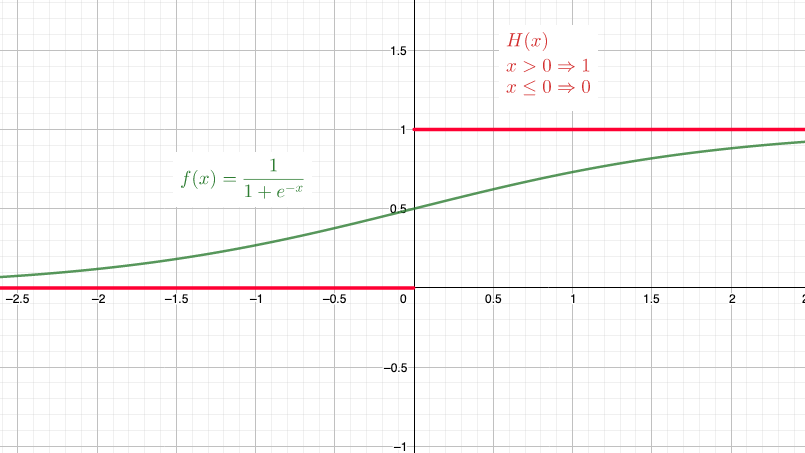
\includegraphics{figures/sigmoid_vs_heaviside.png} \emph{The heaviside
function in red, and the sigmoid function in green}

Let's consider a CNE model, where we use as constraints the degrees of
each nodes, as well as other features. The CNE expression looks like: \[
Q_{ij} = \sigma \left(2 \gamma +\alpha_i + \alpha_j+  \theta^T x_{ij} - ||z_i-z_j||^2 \right)
\]

In the deterministic CNE expression, the link indicators would then look
like:
\[a_{ij} =h\left(2\gamma +\alpha_i + \alpha_j+  \theta^Tx_{ij} - ||z_i-z_j|| \right)
\]

This has a natural visual interpretation, as shown in the following
image 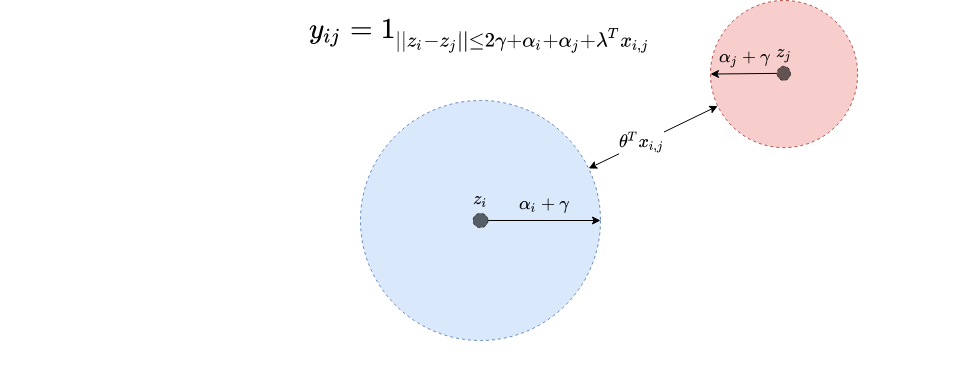
\includegraphics{figures/cne_deg1.png}

As can be seen, each embedding \(z_i\) is endowed with a disk \(D_i\)of
radius \(\alpha_i+\gamma\) such that the minimum distance between
\(D_i\) and \(D_j\) in order for the nodes to connect is
\(\theta^T x_{ij}\).

If the prior similarity is high, the the disk need not be too close for
the connection to form. As a consequence, the embeddings will not encode
the prior information.
